%! suppress = MissingLabel
%! suppress = LineBreak
\section{Разработка игр}

Для демонстрации возможностей системы было разработано два прототипа мобильных 2D игр. 

WebGL сборка проекта и файл APK доступны здесь\cite{s9}. Исходный код доступен в репозитории\cite{s7}.

\subsection{Управление}

{\parindent0pt Для мобильных устройств:}
\begin{enumerate}[label=\textbullet]
    \item Левый джойстик для управления движением.
    \item Правый джойстик для стрельбы.
    \item Жест <<Назад>> для открытия меню паузы.
\end{enumerate}
{\parindent0pt Для ПК:}
\begin{enumerate}[label=\textbullet]
    \item Кнопки WASD для движения.
    \item Правый джойстик для стрельбы.
    \item Кнопка Esc для открытия меню паузы.
\end{enumerate}

\subsection{Игра Shadow Survival}

\textbf{Shadow Survival} -- простая игра в жанре <<Shoot ’em up>>. Во время игры генерируется оружие, которое можно подобрать и настроить некоторые его параметры.

\begin{figure}[ht]
    \begin{center}
        \scalebox{0.22}{
            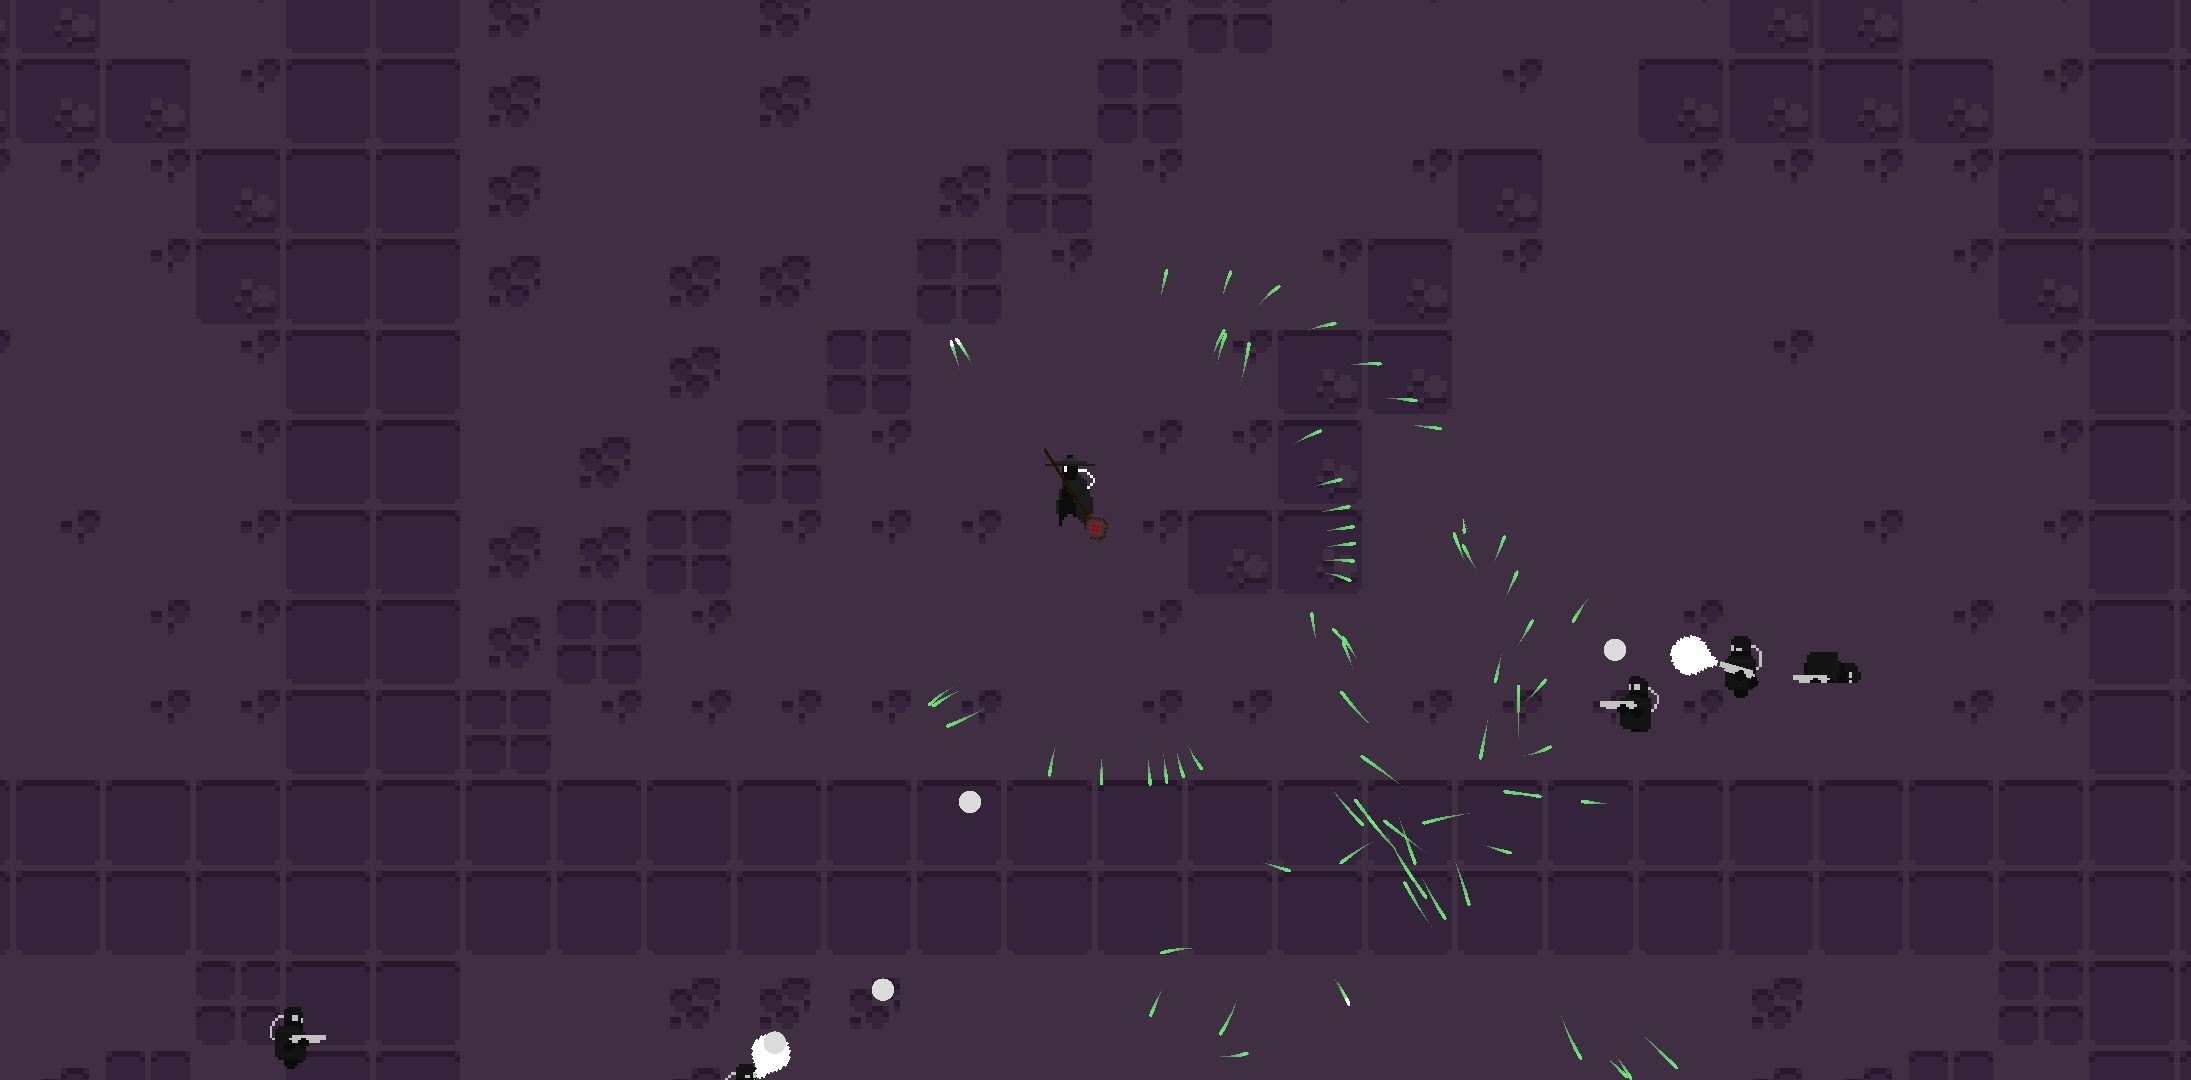
\includegraphics{images/SS}
        }

        \caption{
            \label{ShadowSurvival}
            Shadow Survival.
        }
    \end {center}
\end {figure}

\textbf{Генерация оружия.} В начале игры создаётся случайная популяция из 6 геномов. Каждый такой геном содержится в игровом объекте под названием \textit{Weapon Item} (Рисунок~\ref{WeaponItemIcon}). 

\begin{figure}[ht]
    \begin{center}
        \scalebox{0.08}{
            
\includegraphics{images/WeaponItemIcon}
        }

        \caption{
            \label{WeaponItemIcon}
            Иконка Weapon Item.
        }
    \end {center}
\end {figure}

При контакте \textit{Weapon Item} с игроком активируется окно выбора оружия (Рисунок~\ref{SSCanvas}). В этом окне демонстрируется оружие, содержащееся в данном \textit{Weapon Item}, и есть кнопки для принятия этого оружия или отказа от него.

Кроме того, в окне выбора оружия есть слайдер \textit{Distance}, который позволяет менять параметр {\small \textbf{NNControlDistance}}, и кнопка-флажок \textit{Flip}, меняющая значение параметра {\small \textbf{SignY}} на противоположное.

\begin{figure}[ht]
    \begin{center}
        \scalebox{0.22}{
            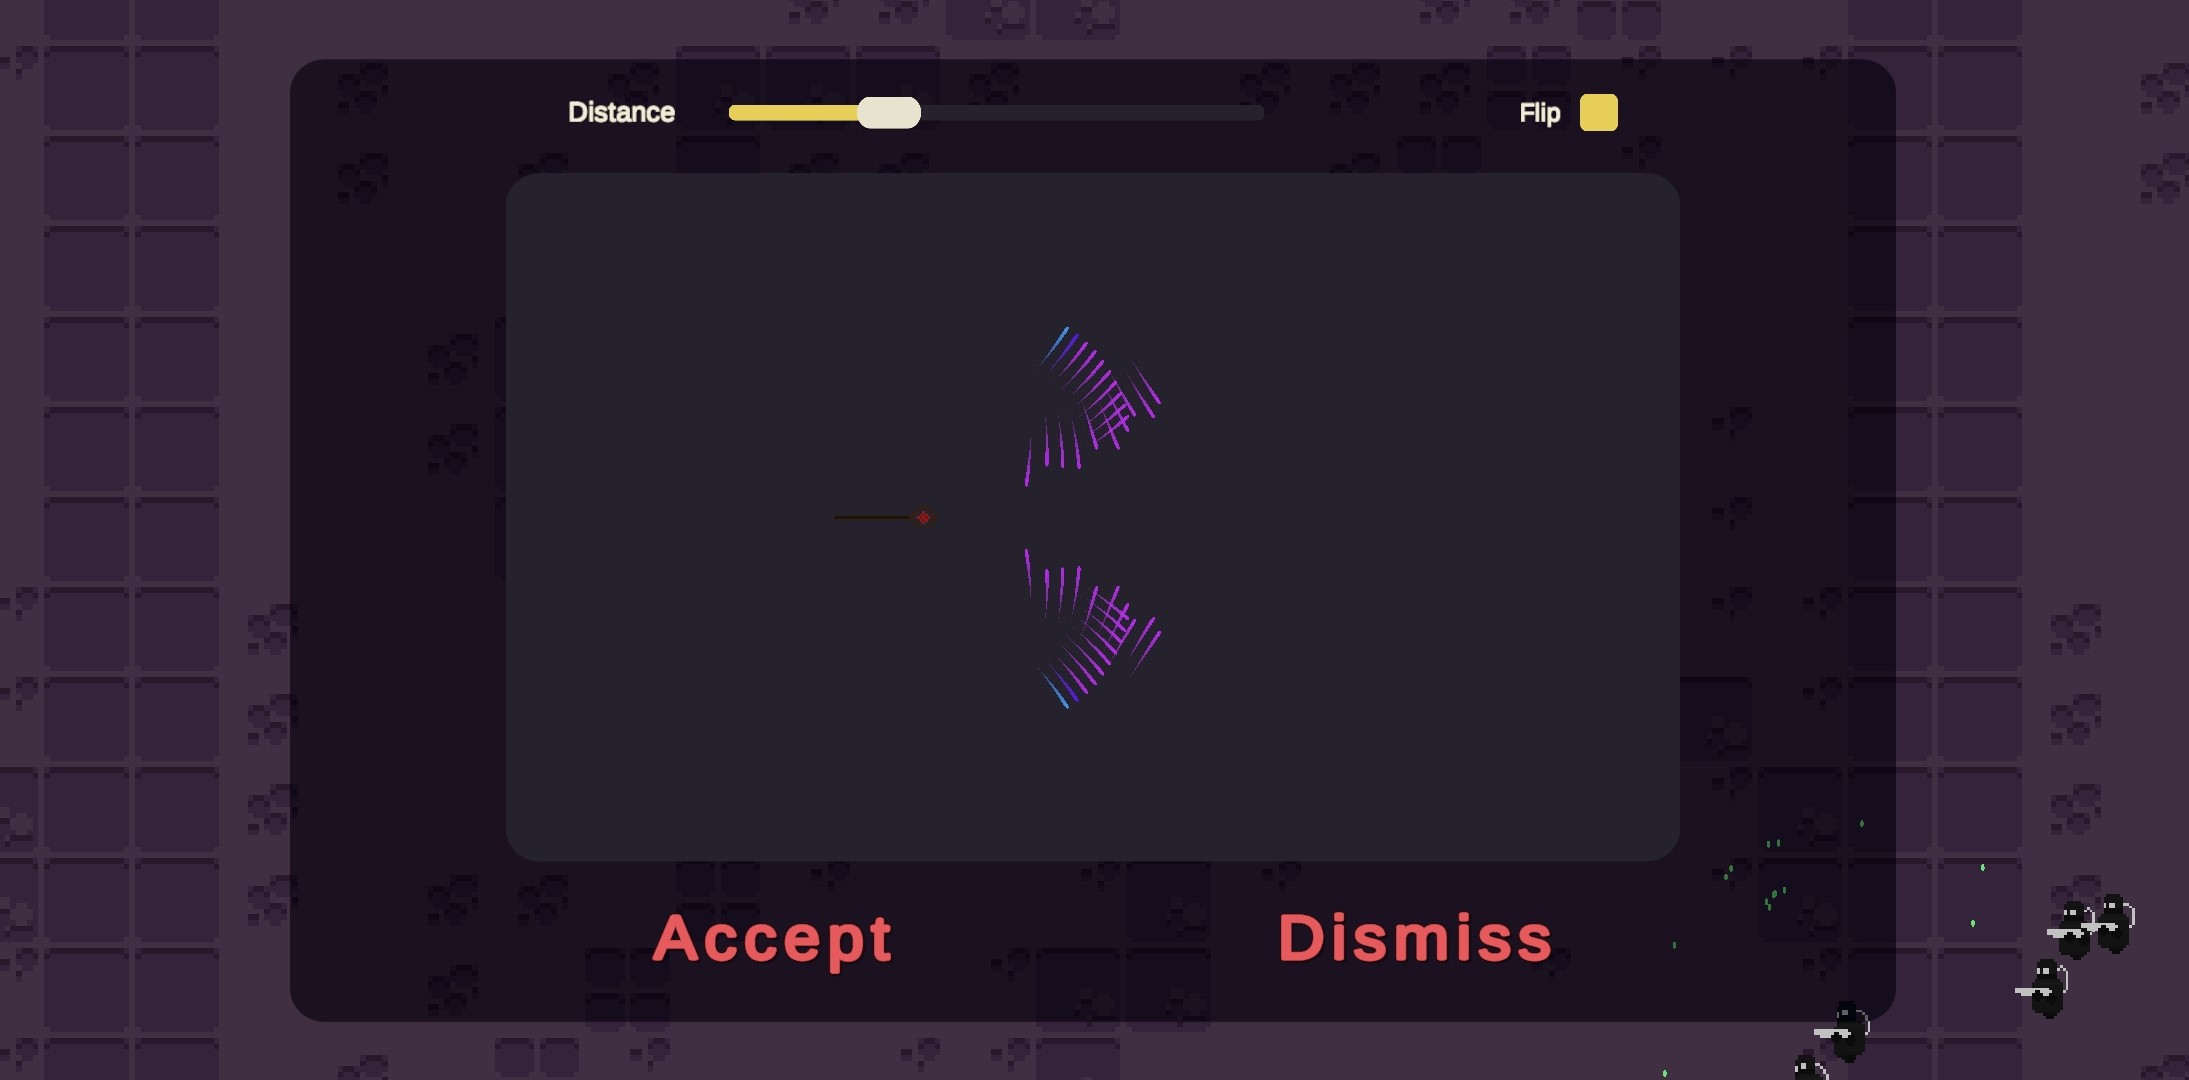
\includegraphics{images/SSCanvas}
        }

        \caption{
            \label{SSCanvas}
            Окно выбора оружия.
        }
    \end {center}
\end {figure}

После того как игрок принял оружие, алгоритм генерирует новое поколение из 6 \textit{Weapon Item}, содержащих 6 новых геномов. Для этого геном только что выбранного оружия скрещивается с геномами не выбранного оружия, в результате чего получается 5 оружий. Ещё одно дополнительное оружие случайным образом выбирается из стартового набора с 140 оружиями, заранее сгенерированными разработчиком.

Таким образом игрок способен влиять на генерацию оружия своим выбором, и при этом он всегда имеет шанс получить хорошее оружие из стартового набора и тем самым разнообразить популяцию. Благодаря этому риск того, что эволюция зайдет в тупик, то есть будет производить одинаковые оружия, значительно снижается.

\subsection{Игра Space Shooter}

\textbf{Space Shooter} -- простая игра тоже в жанре <<Shoot ’em up>>. Здесь оружие генерируется у врагов случайным образом.

\begin{figure}[ht]
    \begin{center}
        \scalebox{0.2}{
            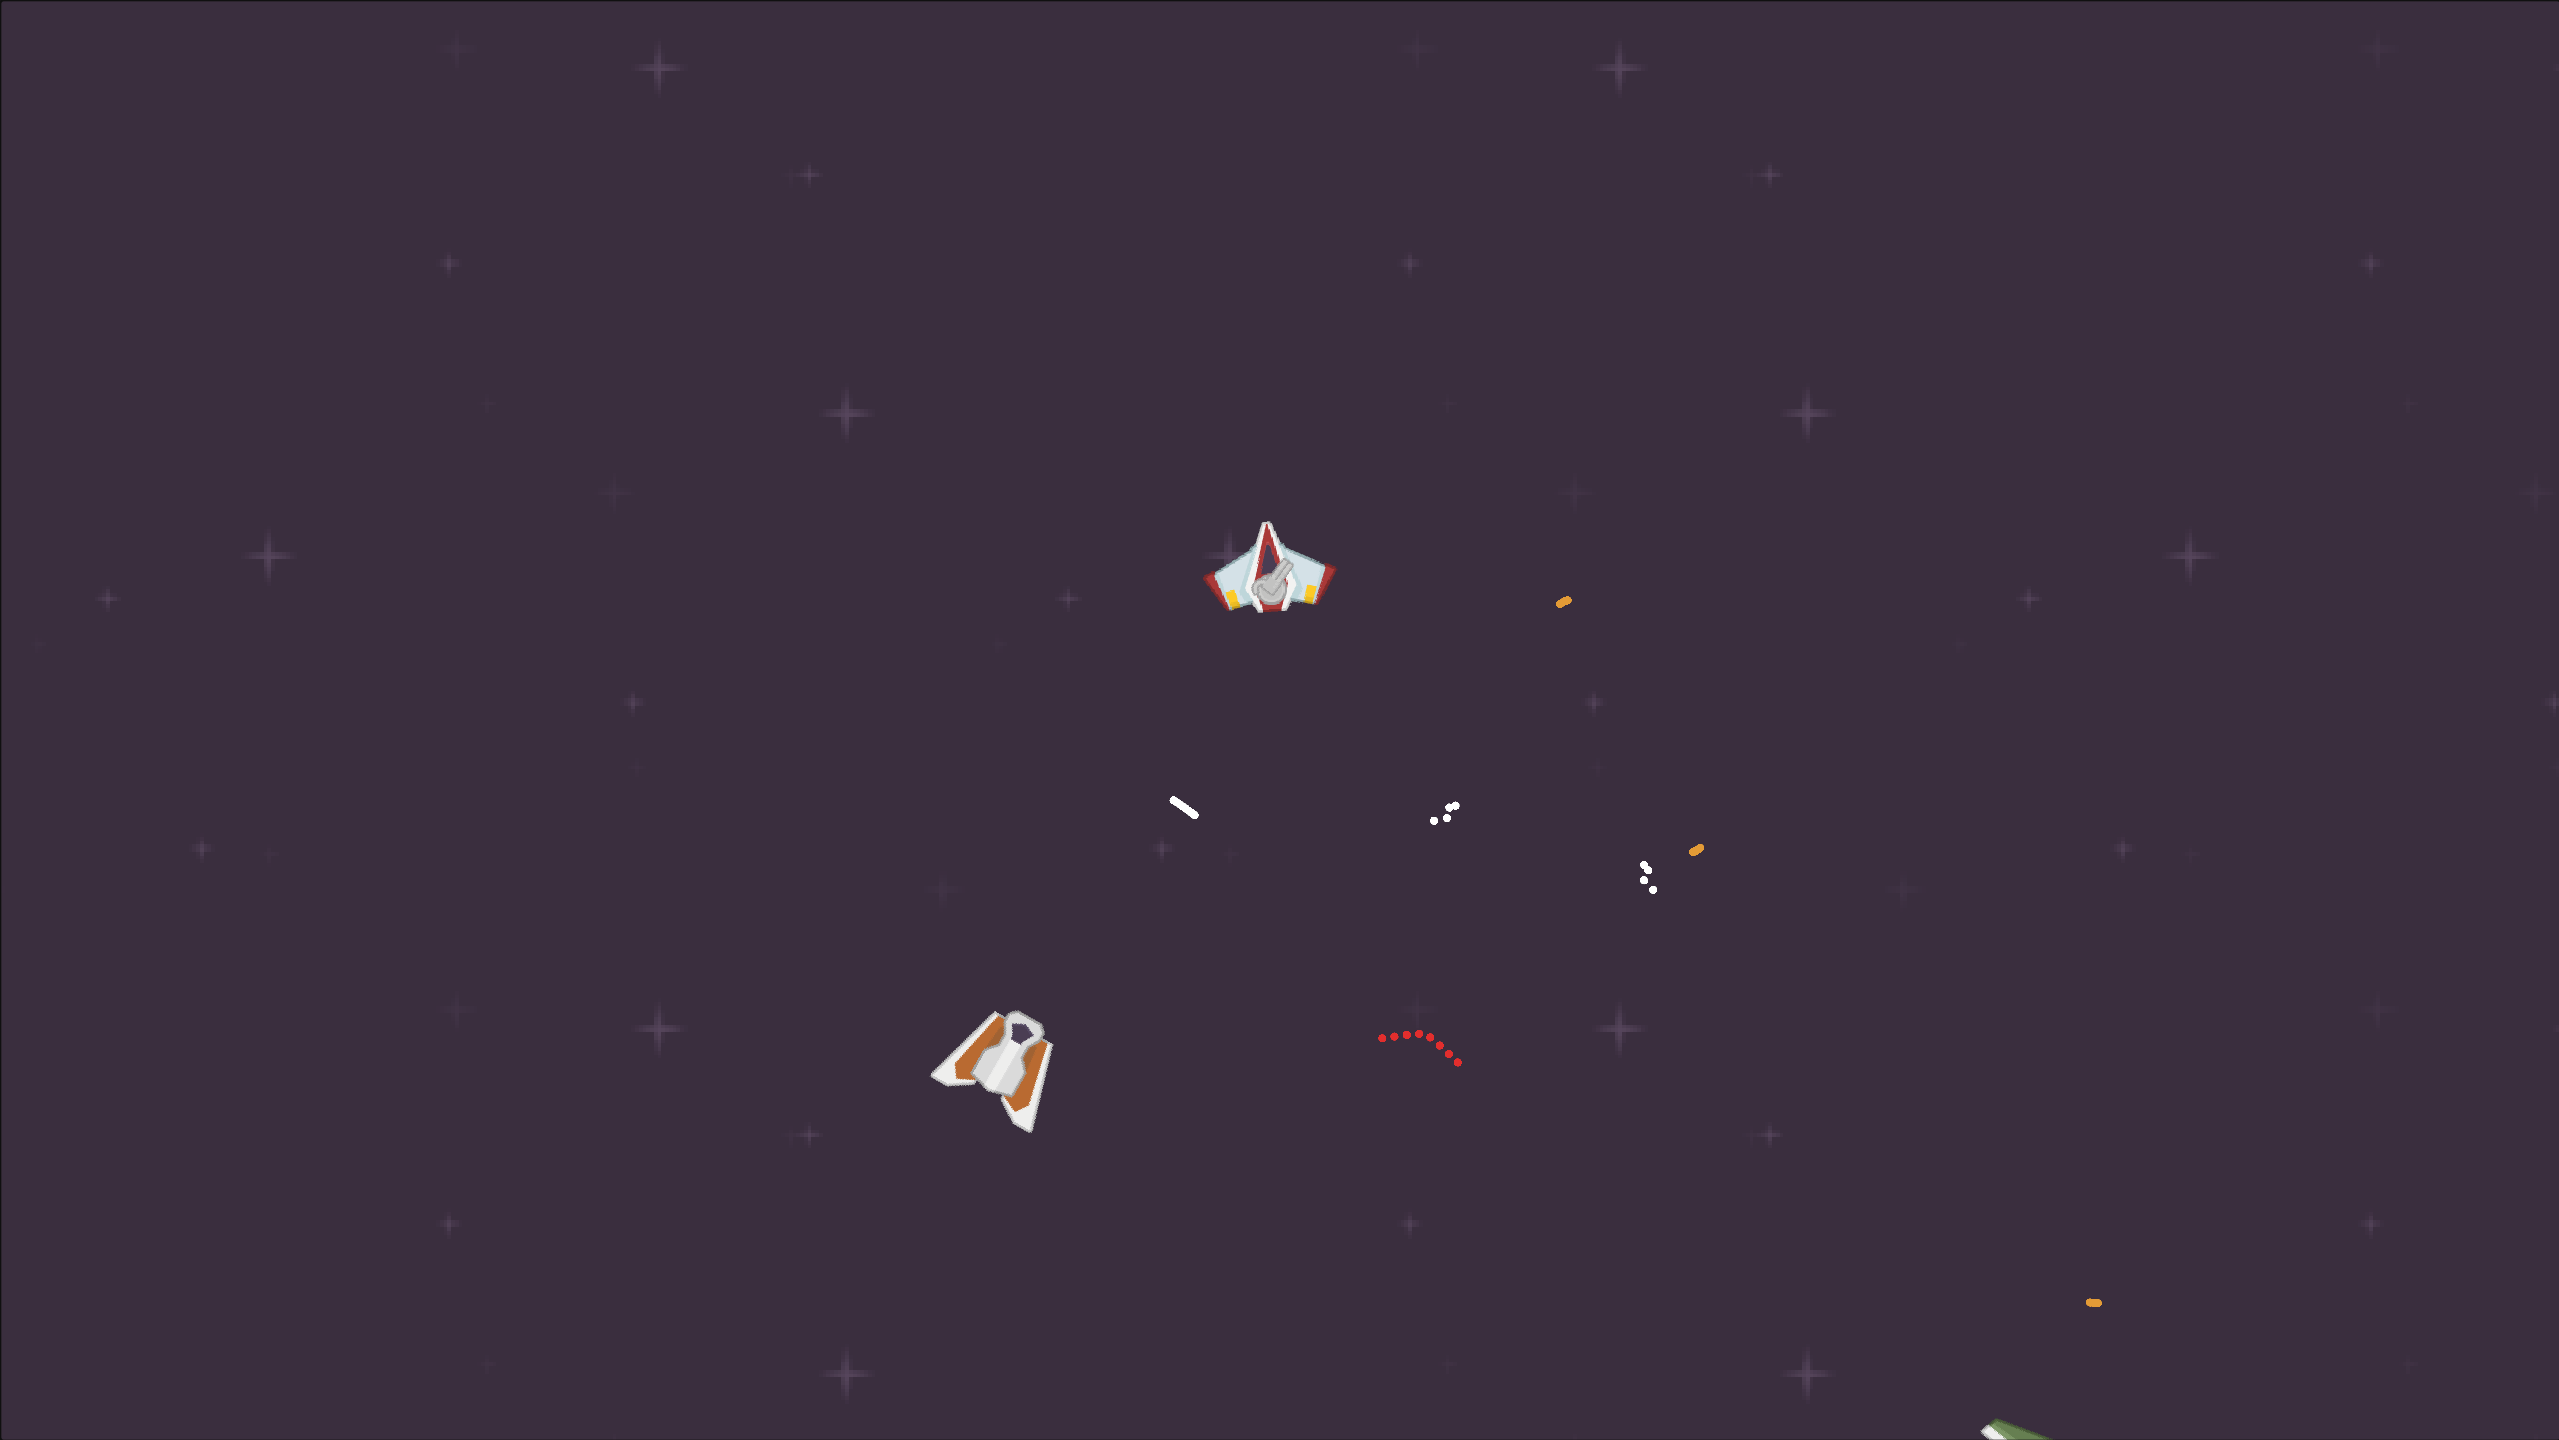
\includegraphics{images/SpaceShooter}
        }

        \caption{
            \label{SpaceShooter}
            Space Shooter.
        }
    \end {center}
\end {figure}

\pagebreak
